% Executive Overview — Hyperspectral Event Sensing: Where We Stand
% Compile: pdflatex executive_overview_2026-09-26.tex (twice, for cross-references)
% ==============================================================================
% Author:        Richard G. Baird
% Date Modified: 2026-09-26
% Notice:        This file was authored or modified with the assistance of
%                Kilo CLI (GLM, z-ai/glm-5.3-flash).
% ==============================================================================
\documentclass[11pt,a4paper]{article}

\usepackage[T1]{fontenc}
\usepackage[utf8]{inputenc}
\usepackage{lmodern}
\usepackage[margin=2.2cm,top=2.4cm,bottom=2.6cm]{geometry}
\usepackage{amsmath,amssymb}
\usepackage{booktabs}
\usepackage{graphicx}
\usepackage{xcolor}
\usepackage[font=small,labelfont=bf,skip=4pt]{caption}
\usepackage{microtype}
\usepackage{enumitem}
\usepackage{tgheros}
\usepackage[hidelinks,colorlinks=true,linkcolor=reportblue,urlcolor=reportblue,citecolor=reportblue]{hyperref}

\definecolor{reportblue}{HTML}{1F3864}
\definecolor{accent}{HTML}{2E74B5}
\definecolor{pale}{HTML}{DDEBF7}
\definecolor{warn}{HTML}{B3470A}

\newcommand{\heading}[1]{\subsection*{\color{reportblue}#1}}
\newcommand{\subheading}[1]{\subsubsection*{\color{accent}#1}}

\setlist[itemize]{itemsep=3pt,topsep=4pt}
\setlist[enumerate]{itemsep=3pt,topsep=4pt}

\title{\vspace{-1.2cm}\textsf{\color{reportblue}\Large Executive Overview}\\[2pt]
\textsf{\color{accent}\large Hyperspectral Event Sensing: Where We Stand, in Practice and in Theory}}
\author{\textsf{Rich Baird}}
\date{\textsf{September 26, 2026}}

\begin{document}
\maketitle
\vspace{-1.4cm}

\begin{center}
\fcolorbox{reportblue}{white}{\parbox{0.96\textwidth}{%
\textsf{\textbf{\color{reportblue}At a glance}\quad
On a color display reference target, signed ON$-$OFF estimation takes cross-color
correlation to \textbf{0.78} (green--red \textbf{0.89}), clearing the 80\% target we
set for this phase, and settles the operating rules: total integration time pays,
effective frame rate is free (10--10{,}000~FPS), single frames never suffice. The
optical front end, not the estimator, is the current frontier. Our first superk
illumination was mis-focused --- the beam flooded the frame instead of forming a tight
coded image --- so those early laser-sweep numbers are superseded; the replacement
display capped the scene at 60~Hz. We have returned to the superk with a corrected
front end: a collimated beam projected onto a translucent screen gives a perfectly
divergent source the lens cannot focus to a point, with the Coded Events-derived
diffractive element in the beam and a 960~rev/s chopper as the temporal probe.
Captures exist; the first analysis pass is dominated by the chopping structure and
awaits signed reprocessing. In theory, the 4D Fisher-information derivation was
audited and corrected (point-process likelihood over signed timestamps,
identifiability first), and it prescribes the decisive test --- reference-gated
readout of the coded mask --- for which practice already has the hardware.}}}
\end{center}

\vspace{0.2cm}

% ============================================================
\heading{1. The concept}

The idea is to make wavelength legible to an event camera through PSF engineering.
A diffractive phase mask in front of the sensor spreads each wavelength into its own
spatial diffraction pattern; chromatic dispersion in the mask means that pattern
changes measurably with wavelength. The spectrum therefore becomes a spatial code on
the sensor, and the task reduces to reading that code from the event stream --- no
filter array, no scan, potentially a full spectral cube per snapshot.

The catch is that event cameras are blind to static intensity. A pixel fires only
when local log-intensity crosses its contrast threshold, so a static scene under
static optics produces no events at all, and a pure global brightness change carries
no spatial code. The system therefore needs a temporal probe --- known motion,
modulation, or gating --- for the coded pattern to express itself in the event
record. That requirement drives most of our experimental design, and it is where the
current bottleneck sits.

The optical element is real: a diffractive optical element designed according to the
Coded Events theory is in the beam path of the current setup, so the sensor sees a
coded PSF rather than a bare spot. What the in-beam element does \emph{not} yet carry
is a design objective aimed at wavelength: Coded Events optimizes the PSF for
event-based encoding in general (tracking, in their setting), while optimizing it
specifically for spectral information under the corrected framework of Section~4 is
future work (Section~6, step~6).

The synthesis itself --- wavelength-coded optics read out by an event camera --- has
not been demonstrated before. Majumder et al.\ (Optica 2025) establish diffractive
snapshot spectral imaging for frame cameras; Shah et al.\ (CVPR 2024, CodedEvents)
establish optimal PSF engineering for event cameras in the 3D-tracking setting and
supply the design theory behind our in-beam element. Our contribution is the
combination, guided by an information-theoretic design criterion described in
Section~4.

% ============================================================
\heading{2. What practice has established}

The pipeline works end to end, with one optical caveat that shaped this phase. Our
first illumination attempt with the superk continua laser was mis-focused: the beam
was not brought to a correct focus, and the camera frame filled with light rather
than forming a tight coded image. That made the original narrowband sweep
(425--675~nm) unusable as a spectral measurement, so we switched to a color display
target for simplicity. The display capped the scene at its 60~Hz refresh
(Section~3), but it provided clean data for settling the estimator and integration
questions --- sensor-level facts that hold regardless of the optical front end:

\begin{itemize}
\item \textbf{Signed polarity binning was the fix.} Counting ON and OFF events
      separately (ON$-$OFF, the scheme CodedEvents proves approximates the
      log-intensity change) raised the converged cross-color correlation from 0.61 to
      \textbf{0.78} on the display target --- blue--green 0.71, blue--red 0.74,
      green--red \textbf{0.89} --- so every pair now clears the 80\% separation
      target. It also removed a spurious trend: the earlier folded-polarity estimator
      showed an apparent 11.6\% frame-rate dependence, which was an artifact of
      folding the two polarities together before a nonlinearity.
\item \textbf{Total integration time is the operative variable.} At fixed total
      averaging time, correlation is flat in effective frame rate (10 to 10{,}000~FPS,
      0.5--2\% spread); it grows only with $T$ (0.5~s: $\approx 0.16$; 5~s: 0.78).
      Frame rate is a free knob; duration is not. The operating envelope for reliable
      discrimination is at least 5 averaged frames and at least 0.5--1~s of total
      integration.
\item \textbf{Detection and estimation must not be conflated.} Single events are
      always detected at microsecond resolution --- that is what the sensor is for.
      But the coded pattern is an estimand, and a single binned frame is one
      threshold-quantized sample of it: 1--2-frame reconstructions deviate by up to
      0.74 in correlation units, while five or more averaged frames converge to
      within 0.075. This mirrors CodedEvents' own no-accumulation ablation
      (+45--54\% tracking RMSE).
\end{itemize}

One caution travels with these numbers: they demonstrate the \emph{estimator}, not
yet the coded optics. The 80\% target was met on display colors; demonstrating it on
laser lines through the coded diffractive element is precisely the job of the
corrected superk setup described next.

\begin{figure}[htbp]
\centering
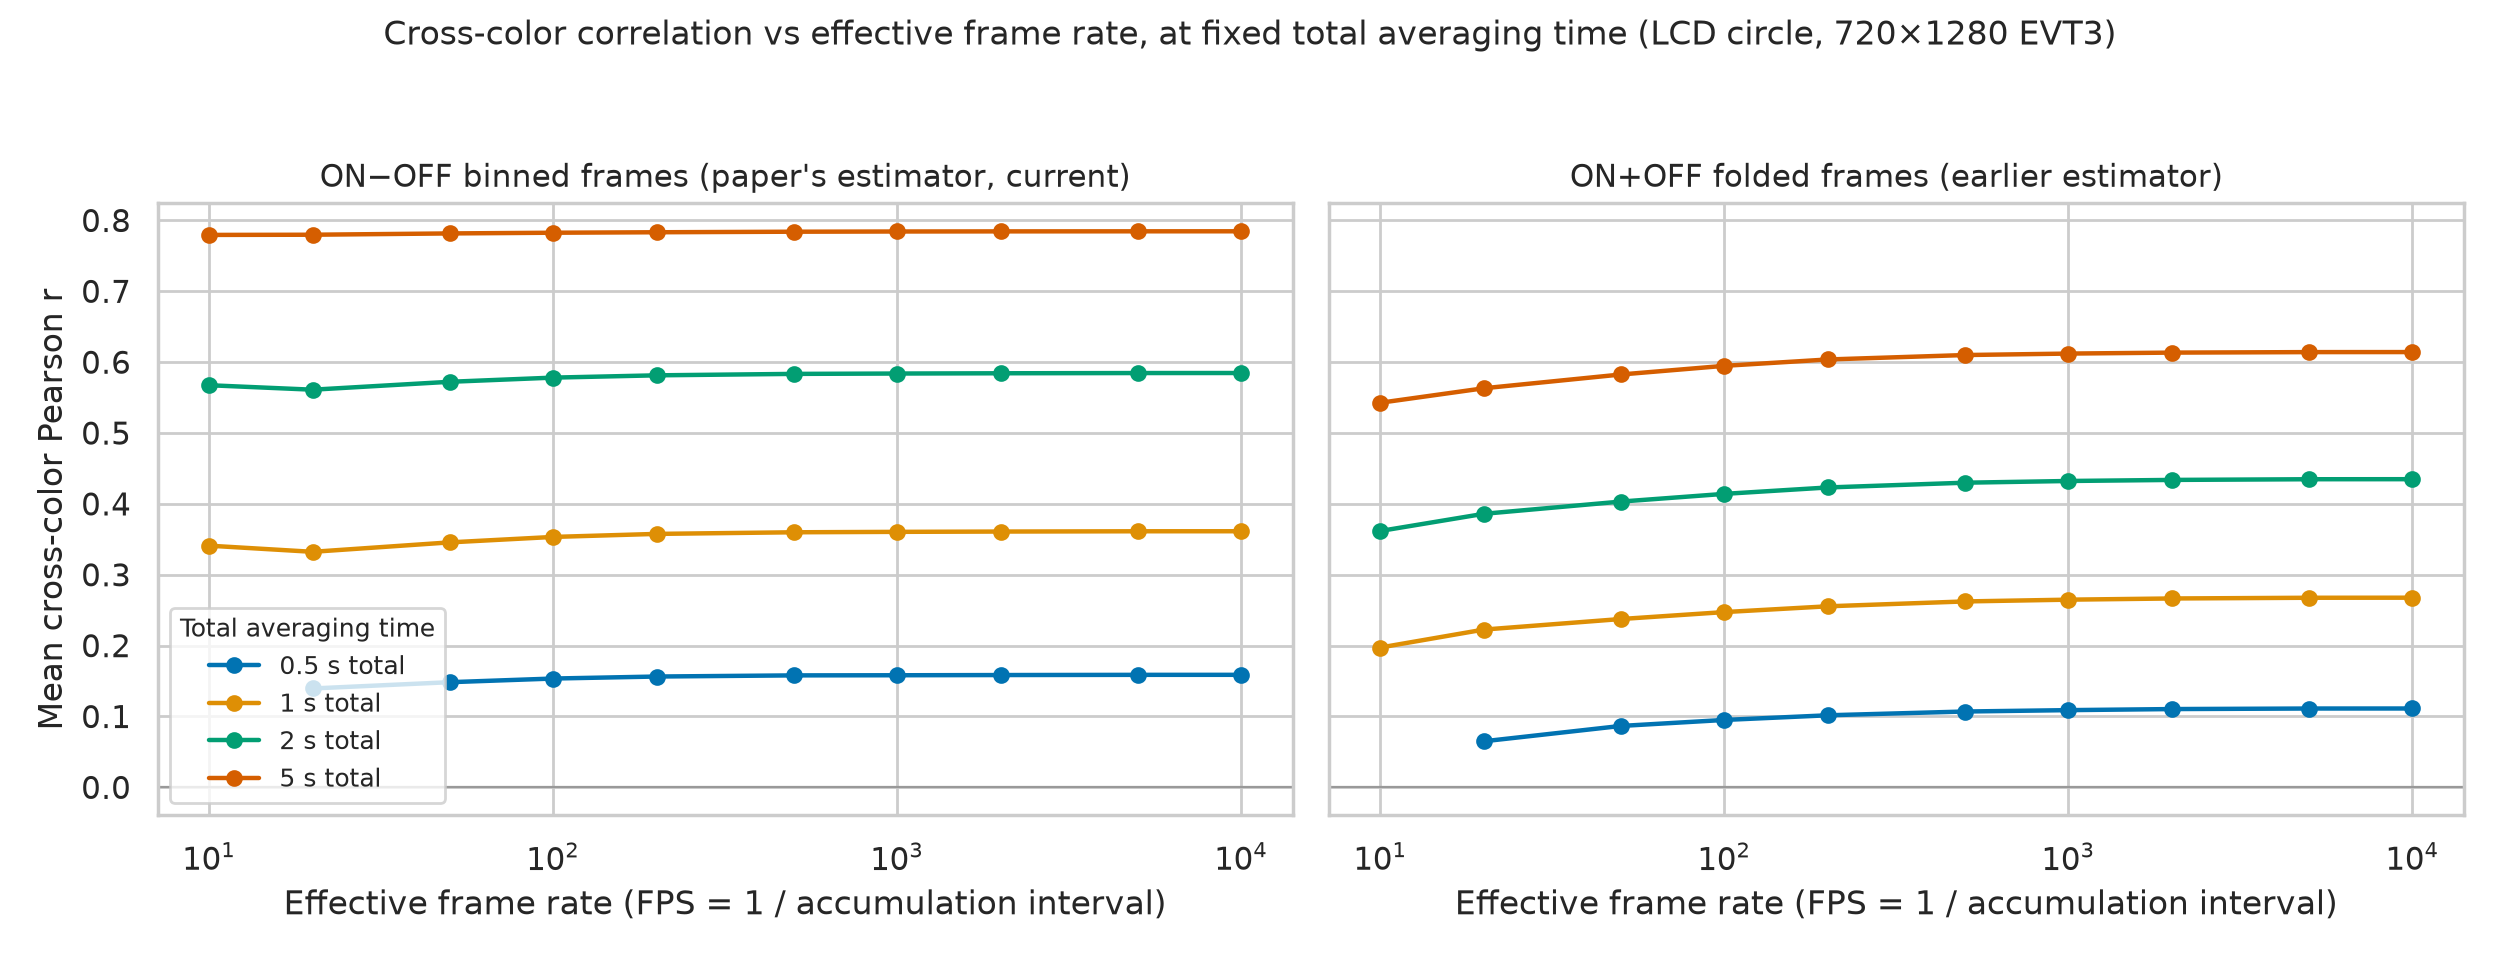
\includegraphics[width=0.98\textwidth]{figures/cross_correlation_vs_effective_frame_rate.png}
\caption{The headline measurement, taken on the color display reference target
(red/green/blue circles). Each line is a fixed total observation time (0.5 to
5 seconds); the horizontal axis is the effective frame rate (the inverse of the
accumulation interval). The curves are flat, so frame rate buys nothing at fixed
total time; the vertical separation between curves shows that integration time is
what pays. The right panel shows the earlier folded-polarity estimator, where the
apparent frame-rate trend lived; that trend was a processing artifact.}
\end{figure}

% ============================================================
\heading{3. Where practice stands now}

\subheading{Why we left the display: the 60~Hz ceiling.} The display target was a
deliberate detour --- simple to drive, clean to analyze --- but it caps scene
dynamics at one refresh period and injects its own periodic modulation into the data.
The signature is a split-half reliability diagnostic that goes negative when analysis
windows sample fixed phases of the display-periodic flicker. On this source we
cannot measure how the minimum usable accumulation window scales with modulation
frequency, which is precisely the design question for the spectroscopy experiments.

\subheading{The corrected superk front end, with the chopper as temporal probe.} We
have moved back to the laser with the illumination failure fixed. A collimated
superk beam is projected onto a translucent screen, producing a perfectly divergent
(diffuse) source --- the lens can no longer focus the beam to a point, which was the
failure mode of the first attempt. The Coded Events-derived diffractive element sits
in this beam path, so the sensor now sees the coded PSF under correctly divergent
illumination. To supply the fast temporal probe the display could not, the 12-window
chopper wheel (960~rev/s, 11.52~kHz per-pixel chop, constant aggregate flux)
modulates the scene, and recordings exist across 475--675~nm.

The first analysis pass on those captures is, honestly, not yet a result: processed
with the legacy folded polarity and without trigger alignment (the photodiode
sidecars came back empty during capture), the shared chopping structure dominates and
cross-color correlation saturates around 0.97. The rework path is clear --- signed
ON$-$OFF binning, integration aligned to whole revolutions, then a frequency ladder
(97/211/503~Hz, deliberately incommensurate with 60~Hz, plus one commensurate
control and a chopper-off baseline). The prediction on the table: the minimum usable
accumulation window scales as $t_{\min} \propto 1/f$, equivalently results from all
speeds collapse onto one curve in events-per-window. If it holds, that scaling is
the design map connecting scene dynamics to camera settings --- and the reprocessed
captures will be the first true test of laser-line discrimination through the coded
element.

% ============================================================
\heading{4. Where theory stands}

The role of theory is to compute, before any optics are fabricated, the Fisher
information the optical design delivers and the Cram\'er--Rao lower bound that follows
from it --- the best accuracy any unbiased estimator could achieve for a given mask,
probe, and photon budget. Our first manuscript derived a 4D Fisher-information matrix
over space, time, and wavelength (source velocity, intensity shift, and spectral shift
jointly with mask phase and PSF geometry), which is the right target and more general
than CodedEvents' two-time-position model.

A technical response note then audited the derivation. The audit keeps the goal and
the Poisson count algebra but corrects the load-bearing parts:

\begin{itemize}
\item \textbf{The likelihood was wrong in kind, not just in parameters.} Photon
      arrivals being Poisson does not make camera events Poisson; a noiseless log
      ramp fires periodic events. The correct object is a point-process likelihood
      over signed, timestamped events, including the survival integral --- the
      information carried by the \emph{absence} of events. Binned counts, the basis
      of the original derivation, discard exactly the timing information this
      framework preserves.
\item \textbf{The joint matrix was presented before it was earned.} The 9$\times$9
      ``hyperspectral'' Fisher matrix (reported condition number
      $3.9 \times 10^{19}$) is a symbolic construction, not a derived bound: a
      spectrum needs multiple spectral coefficients with an incoherent intensity sum
      before the logarithm, a near-sensor diffractive element is generally
      space-variant rather than a shift-invariant PSF, and identifiability ---
      Jacobian rank, rescaling, nuisance-parameter marginalization --- must be
      established before anything can be inverted or claimed.
\item \textbf{The illumination-scaling claim is conditional, not a law.} The
      derivation argued that the event-camera bound worsens linearly with photon
      count (implying an optimal low-light operating point, in contrast to frame
      cameras). The audit shows the brightness cancellation it relied on is a
      property of a particular noise-free model; no universal CRLB-versus-$N$
      scaling or low-light optimum follows without separating source intensity,
      background, and threshold noise on calibrated hardware.
\item \textbf{A useful identifiability caution.} Under certain conditions absolute
      brightness is unobservable from events alone (scale invariance under a global
      gain with zero reference). The acquisition must therefore anchor brightness ---
      reference gating --- or fix a scale gauge and estimate normalized spectral
      shape.
\end{itemize}

The response note is constructive: it supplies the corrected likelihood, the spectral
sensitivity operator (verified against independent numerical differentiation to
$1.8 \times 10^{-10}$ relative error in a three-band test), and the design objective
--- minimize the trace of the inverse effective Fisher information over design
scenes. The net position: we have an agreed, correct framework; what we do not yet
have is a \emph{numerical} bound, because that requires the calibrated optical
forward model first.

% ============================================================
\heading{5. How the two tracks connect}

Both documents independently nominate the same decisive experiment. On the practice
side it appears as the next bench test; on the theory side it is the acceptance
criterion in the response note's closing section: \textbf{reference-gated
acquisition} --- modulate or gate the scene against a calibrated, nonzero additive
reference (never a zero baseline inside the logarithm), under fixed known motion ---
and then test whether the spectrally coded spatial pattern survives event conversion.
Practice already has the hardware and the split-half noise-ceiling machinery to
score the result; theory specifies the analysis (effective Fisher information after
marginalizing nuisance parameters, Jacobian-rank checks) and the ground truth
(held-out spectral mixtures against a spectrometer). Dither versus gating is the
first comparison; it answers directly whether the designed code survives the sensor.

\begin{center}
\fcolorbox{warn}{white}{\parbox{0.96\textwidth}{%
\textbf{\color{warn}Highest technical risk}\quad
Whether the wavelength coding of the in-beam diffractive element survives event
conversion strongly enough to discriminate --- and ultimately reconstruct ---
laser lines. The mitigation is ordering: the chopper captures already in hand
(reprocessed, step~1) and the reference-gating test (step~4) answer this with the
existing element, before any spectrally optimized redesign is fabricated.}}
\end{center}

% ============================================================
\heading{6. Next steps, in order}

\begin{enumerate}
\item \textbf{Reprocess the chopper recordings} with signed ON$-$OFF binning and
      revolution-aligned integration. This is the first genuine test of laser-line
      discrimination through the coded element under the corrected illumination.
      Days; existing data.
\item \textbf{Run the frequency ladder} (incommensurate speeds plus a 60~Hz-commensurate
      control and a chopper-off baseline) and test $t_{\min} \propto 1/f$ /
      events-per-window collapse. One to two weeks; yields the design map.
\item \textbf{Calibrate the diffractive forward model on measured data and recompute
      the bound} --- effective Fisher information with nuisance blocks, identifiability
      first --- replacing the corrected-on-paper but still non-numeric theory result.
      Two to three weeks; no new hardware.
\item \textbf{The reference-gating experiment}: does the coded pattern survive event
      conversion? The project's go/no-go milestone, immediately after 1--2.
\item \textbf{Reconstruct an actual spectrum} against spectrometer ground truth,
      moving the deliverable from pairwise discrimination to spectral estimation.
\item \textbf{Optimize the diffractive element for spectral information}: the in-beam
      design follows the Coded Events theory; re-derive the mask objective for
      wavelength coding under the corrected framework, fabricate, and repeat
      steps 4--5 with it in the beam.
\end{enumerate}

% ============================================================
\heading{7. Bottom line}

\textbf{Demonstrated:} the estimator and its operating rules --- signed ON$-$OFF
estimation takes the display reference target to 0.78 cross-color correlation
(0.89 green--red), clearing the 80\% target, with integration time paying, frame
rate free, and single frames never sufficient. \textbf{Not yet demonstrated:}
laser-line discrimination through the coded diffractive element under the corrected
illumination (chopper captures in hand, analysis awaiting the signed rework),
spectral reconstruction, and a mask optimized for wavelength coding. \textbf{In
theory:} the 4D derivation set the right target and the audit rebuilt it on correct
footing --- point-process likelihood over signed timestamps, identifiability before
inversion --- so the framework is agreed and its central equation verified, with a
numerical bound now waiting only on the calibrated forward model that step~3
delivers.

\end{document}
